\newpage
\section{GIAO DIỆN NGƯỜI DÙNG VÀ DEMO SẢN PHẨM}

\subsection{Demo sản phẩm}

Link video Demo sản phẩm trên Google Drive: \url{https://drive.google.com/file/d/1Nr93MCFbsciDFKg_xInyUwdJTMvygbvV/view?usp=sharing}

Mã nguồn báo cáo \LaTeX, Mã nguồn Web App, Mã nguồn Yolo:bit và IoT Gateway: \url{https://github.com/yymt242/DADN242_Group82}

\subsection{Chạy hệ thống}

\begin{enumerate}[label=\textbf{Bước \arabic*.}, leftmargin=1.5cm]

    \item \textbf{Truy cập giao diện điều khiển web}

          Mở trình duyệt và truy cập trang web điều khiển được host tại địa chỉ:
          \begin{center}
              \url{https://yymt242.github.io/DADN242_Group82/}
          \end{center}

          Đăng nhập bằng tài khoản quản trị viên:

          \begin{lstlisting}[style=pythonstyle]
    Email:    admin1234@hcmut.edu.vn
    Mật khẩu: admin1234
    \end{lstlisting}

    \item \textbf{Nạp chương trình cho thiết bị Yolobit}

          \begin{itemize}
              \item Sử dụng trình duyệt Google Chrome.
              \item Truy cập trang lập trình Yolobit: \url{https://app.ohstem.vn/}
              \item Tiến hành:
                    \begin{enumerate}
                        \item Cập nhật firmware cho thiết bị.
                        \item Cài đặt thư viện mở rộng cần thiết.
                        \item Reset thiết bị bằng cách: Nhấn giữ nút A trong 3 giây, sau đó nhấn nút Reset trong 1 giây (vẫn giữ nút A), rồi thả nút A.
                        \item Nạp chương trình đã được chuẩn bị.
                    \end{enumerate}
          \end{itemize}

    \item \textbf{Khởi động chương trình IoT Gateway trên máy tính (Windows)}

          Mở terminal (CMD hoặc PowerShell), chạy lần lượt các lệnh sau để cài đặt và chạy:

          \begin{lstlisting}[style=pythonstyle]
    py -m pip install --upgrade pip
    pip install requests pyserial
    py .\gateway.py
    \end{lstlisting}

          Để dừng chương trình, nhấn tổ hợp phím \texttt{Ctrl + C}.

\end{enumerate}

\subsection{Giao diện người dùng}


\begin{minipage}{0.45\textwidth}
    \begin{figure}[H]
        \centering
        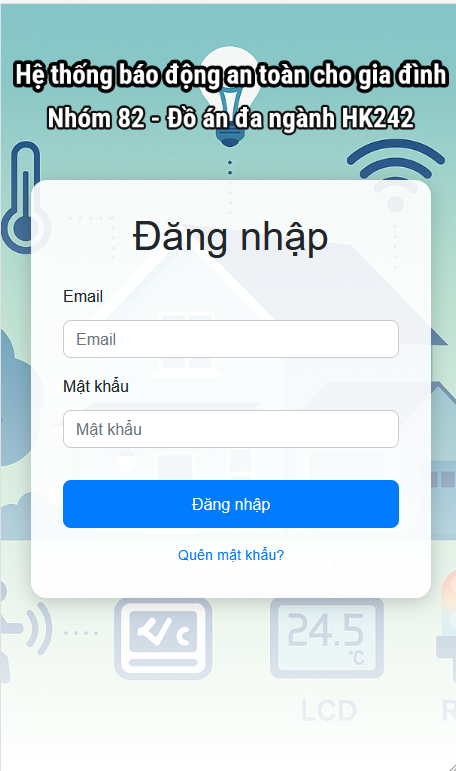
\includegraphics[height=9cm]{figures/dangnhap.png}
        \caption{Giao diện trang đăng nhập}
        \label{fig:dangnhap}
    \end{figure}
\end{minipage}
\hfill
\begin{minipage}{0.45\textwidth}
    \begin{center}
        \begin{figure}[H]
            \centering
            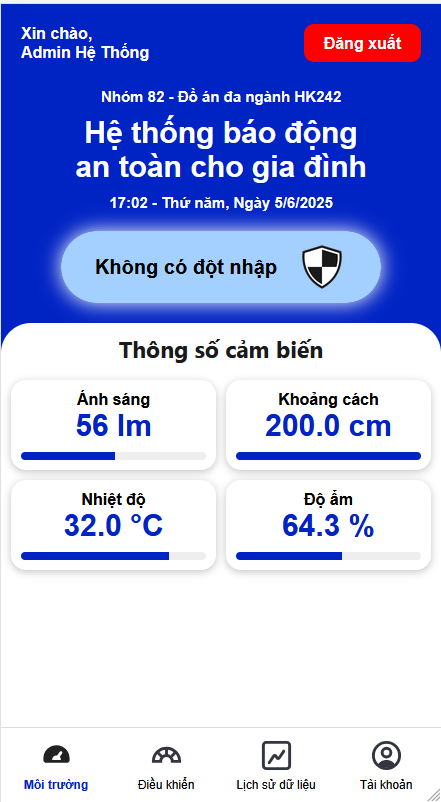
\includegraphics[height=9cm]{figures/moitruong.png}
            \caption{Giao diện trang chủ - dữ liệu môi trường, và các tab điều hướng}
            \label{fig:moitruong}
        \end{figure}
    \end{center}
\end{minipage}



\begin{minipage}{0.45\textwidth}
    \begin{figure}[H]
        \centering
        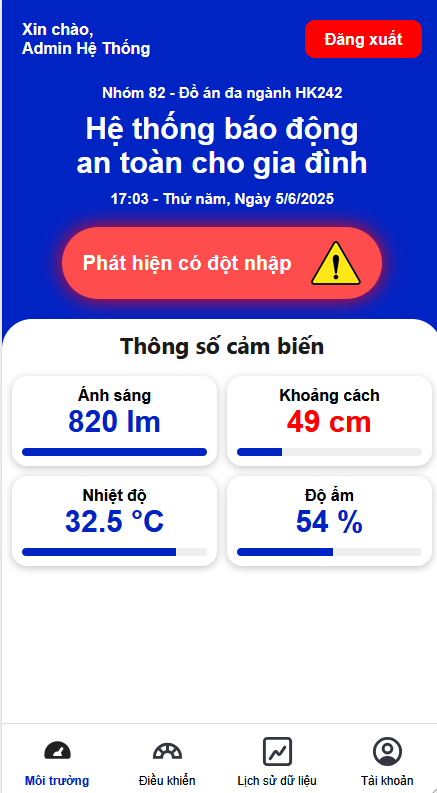
\includegraphics[height=9cm]{figures/dotnhap.png}
        \caption{Giao diện khi có cảnh báo đột nhập}
        \label{fig:dotnhap}
    \end{figure}
\end{minipage}
\hfill
\begin{minipage}{0.45\textwidth}
    \begin{center}
        \begin{figure}[H]
            \centering
            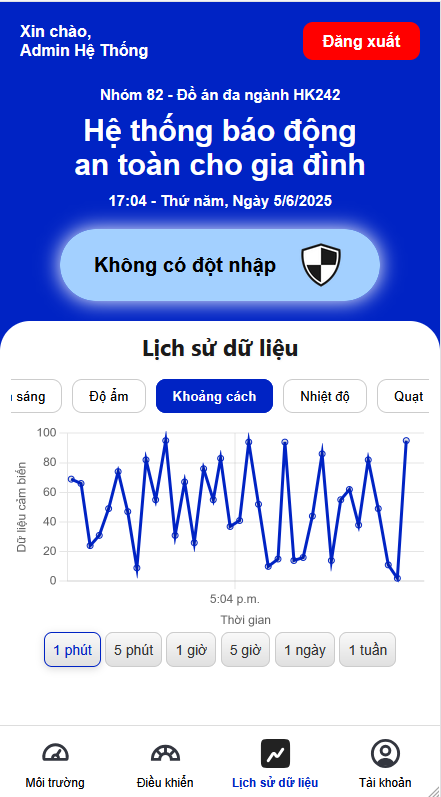
\includegraphics[height=9cm]{figures/dulieu.png}
            \caption{Giao diện xem dữ liệu cảm biến theo thời gian}
            \label{fig:dulieu}
        \end{figure}
    \end{center}
\end{minipage}

\begin{minipage}{0.45\textwidth}
    \begin{figure}[H]
        \centering
        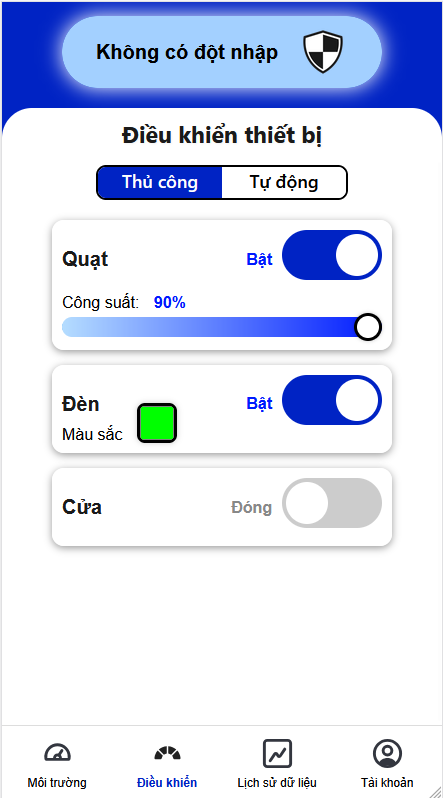
\includegraphics[height=9cm]{figures/thucong.png}
        \caption{Giao diện trang điều khiển thiết bị thủ công}
        \label{fig:thucong}
    \end{figure}
\end{minipage}
\hfill
\begin{minipage}{0.45\textwidth}
    \begin{center}
        \begin{figure}[H]
            \centering
            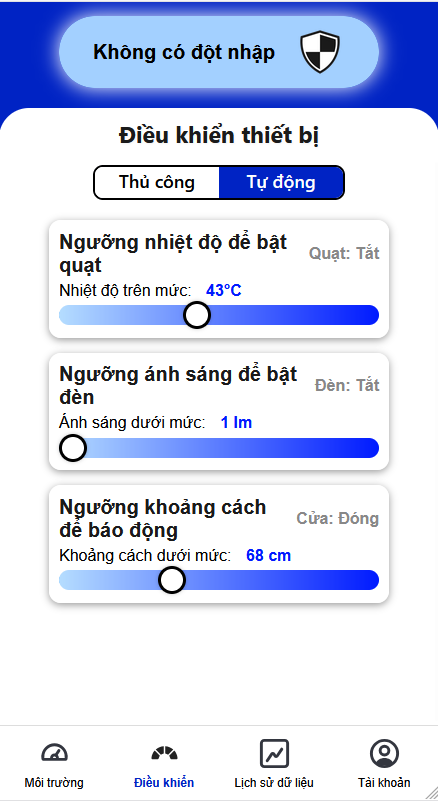
\includegraphics[height=9cm]{figures/tudong.png}
            \caption{Giao diện cài đặt các ngưỡng cho điều khiển thiết bị tự động}
            \label{fig:tudong}
        \end{figure}
    \end{center}
\end{minipage}

\begin{minipage}{0.45\textwidth}
    \begin{figure}[H]
        \centering
        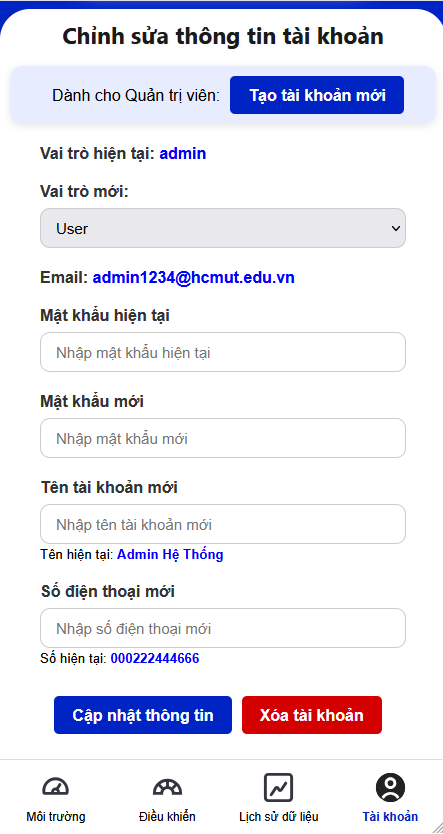
\includegraphics[height=9cm]{figures/taikhoan_chinhsua.png}
        \caption{Giao diện trang chỉnh sửa thông tin tài khoản}
        \label{fig:taikhoan_chinhsua}
    \end{figure}
\end{minipage}
\hfill
\begin{minipage}{0.45\textwidth}
    \begin{center}
        \begin{figure}[H]
            \centering
            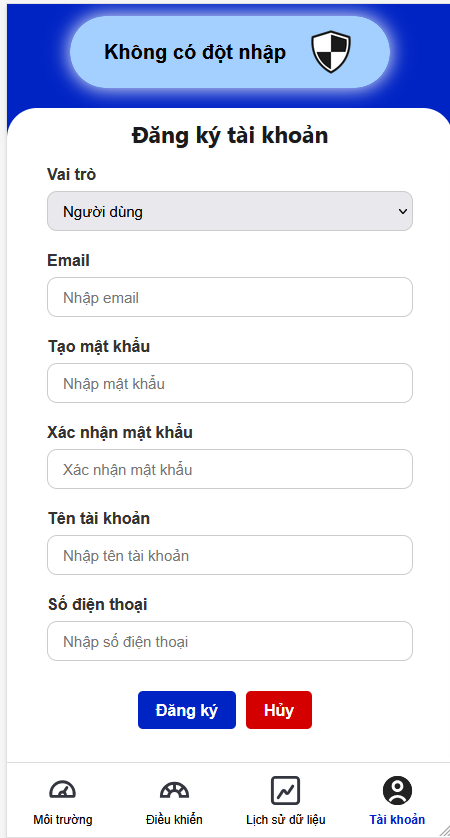
\includegraphics[height=9cm]{figures/taikhoan_dangky.png}
            \caption{Giao diện đăng ký tài khoản mới (Chức năng cho Admin)}
            \label{fig:taikhoan_dangky}
        \end{figure}
    \end{center}
\end{minipage}